\chapter{Evaluation of Neural Network Models} \label{chap:eval_NN}
This chapter examines the applications of Bayesian neural networks using a dataset on housing prices in Boston for regression and a dataset on defaults for credit card clients for classification. We do this using a classic neural network as benchmark for performance to test if it's possible to benefit from the perks of using Bayesian neural networks without sacrificing accuracy and to examine the difference in computational runtime. \\
\\
Section \ref{sec:Boston_housing} examines median prices on houses in specific areas in Boston based on a number of features shown in table \ref{tab:Boston_Housing}. We aim to predict unknown median prices based on these features using regression. Section \ref{sec:credit_default} examines the probability of defaulting payments on credit card users in Taiwan. We aim to predict default or not default and the probabilities of these outcomes using binary classification. We performs these tasks with BNNs with different sampling algorithms and NNs with different regularization methods. We illustrate NNs with different regularization methods to examine the difference in effect of these, for selecting a NN that can serve as a non-overfitting benchmark for the BBNs and to show the hurdles we avoid in Bayesian neural networks. 

\section{Predicting House Prices in Boston} \label{sec:Boston_housing}
The Boston housing was originally introduced by \cite{HARRISON197881}, who investigated the effect of air pollution on house prices. 
The dataset contains information collected by the U.S Census Service concerning housing in the area of Boston Massachusetts. The sample contains 506 examples, where each example represents a unique area and has 14 features. These features are represented in table \ref{tab:Boston_Housing}. The data set can be found on \href{http://lib.stat.cmu.edu/datasets/boston}{http://lib.stat.cmu.edu/datasets/boston}. In this section we examine how to use the theory presented in the previous chapters for predicting the median value of owner-occupied homes in thousands, that is the \texttt{medv} variable in the data set is our target variable. The target variable is a real-valued variable, thus a regression task would be most appropriate.   
Our objective is to make good predictions for house predictions in terms of a low mean squared error (MSE) on unseen data, we therefor split data into a training and testing set respectively, where the training data contains 70\% of the original data and test set the remaining data points. To avoid the possibility that the data is sorted in some undesired way we choose to shuffle the data randomly before splitting it. In order for the reader to be able to regenerate the results we have fixed the state of the underlying pseudo random number generator with a seed. \\
\\
 A predictive model for house prices can be very useful in many applications, for example a Real Estate Investment Trusts (REIT), that wants to invest in real properties and not just the mortgages. A REIT are often inferring Real estate valuation, based on some kind fundamental analysis identical to how fundamental analysis are performed for stock valuation. This process could be substituted with a predictive model instead. The REIT could thus use this model for making quantitative predictions for the right price for a new investment opportunity. Other benefits could be that the REIT can now rely solely on data, instead of relying on a subjective opinion from a fundamental analyst or a real estate agent.   



\begin{table}
\caption{Table of features in Boston Housing data. The dataset contains 506 examples each with 14 features. Data can be downloaded on \href{http://lib.stat.cmu.edu/datasets/boston}{http://lib.stat.cmu.edu/datasets/boston}.}
\label{tab:Boston_Housing}
\centering
\resizebox{\textwidth}{!}{%
\begin{tabular}{|l|l|}
\hline
\multicolumn{1}{|c|}{{\cellcolor{ashgrey}{
 \textbf{Feature name}}}} & \multicolumn{1}{|c|}{{\cellcolor{ashgrey}{
 \textbf{Feature description}}}} \\ \hline
crim              &   Per capita crime rate by town     \\ \hline
zn                &  Proportion of residential land zoned for lots over 25,000 sq. ft                  \\ \hline
indus             &   Proportion of residential land zoned for lots over 25,000 sq. ft                   \\ \hline
chas              & Charles River dummy variable\\
&  (= 1 if tract bounds river; 0 otherwise)   \\ \hline
nox               &  Nitric oxide concentration (parts per 10 million)                    \\ \hline
rm                &   Average number of rooms per dwelling                   \\ \hline
age               &    Proportion of owner-occupied units built prior to 1940                  \\ \hline
dis               &   Weighted distances to five Boston employment centers                   \\ \hline
rad               &   Index of accessibility to radial highways                   \\ \hline
tax               &   Full-value property tax rate per $10,000 $                  \\ \hline
ptratio           &   Pupil-teacher ratio by town                   \\ \hline
b                 & $1000(Bk - 0.63)^2$, where Bk is the proportion of people of   \\ 
& African American descent by town                     \\ \hline
lstat             &    Percentage of lower status of the population                   \\ \hline
medv              &  Median value of owner-occupied homes in $1000s$                    \\ \hline
\end{tabular}}
\end{table}



\subsection{Regression with Neural Networks}
We perform regression with the neural networks listed in table \ref{tab:Boston_NN_performance}. All of these are performed using MSE as loss function, the ReLU activation function in equation \ref{eq:relu} on every hidden layer and no activation function for the output layer. All of the networks have 10 neurons in each hidden layer and train with 300 epochs using ADAM described in section \ref{sec:ADAM}. We have selected these settings as they was found to provide acceptable results after experimentation with several other options. We reuse these settings for all networks to make them more suitable for comparison. 
\\
\\
To examine overfitting in the neural networks we split the data not used for test data into training data and validation data. This in done by a randomized shuffled split that takes 30\% of the remaining data for validation and 70\% for training. The training and validation loss for each training epoch is shown for the networks in figure \ref{fig:Boston_NN_nohidden_wd_loss}, figure \ref{fig:Boston_NN_1hidden_wd_loss} and figure \ref{fig:Boston_NN_1hidden_noreg_loss}.\\

\begin{figure}
    \centering
    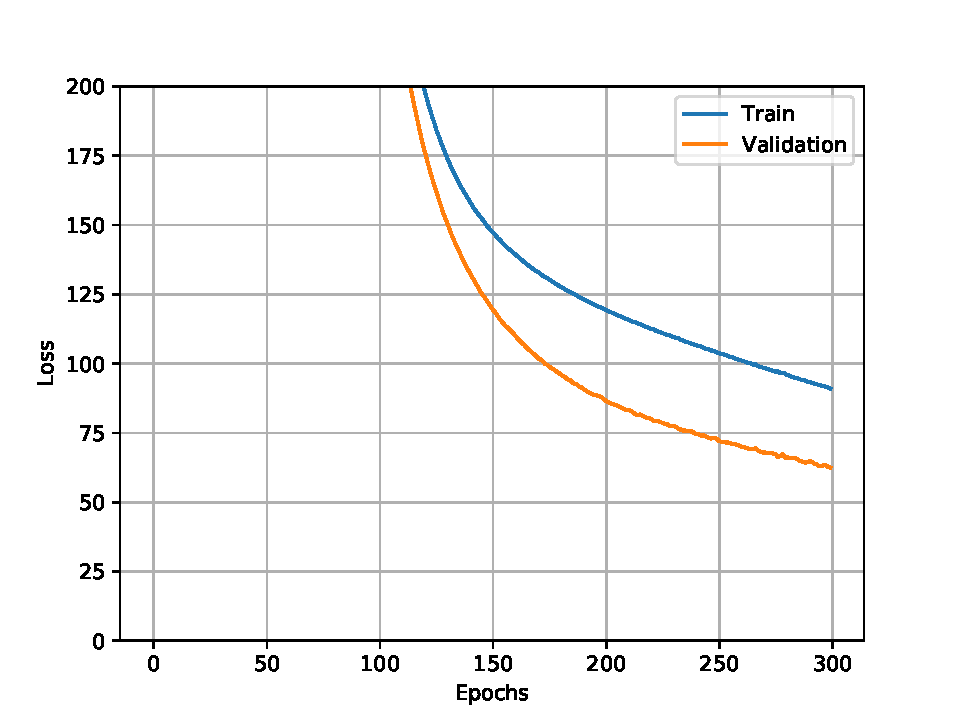
\includegraphics{pics/figure_Boston_NN_nohidden_wd_loss.pdf}
    \caption{Loss on training and validation set during training epochs for the neural network with no hidden layers \& weight decay.}
    \label{fig:Boston_NN_nohidden_wd_loss}
\end{figure}

\begin{figure}
    \centering
    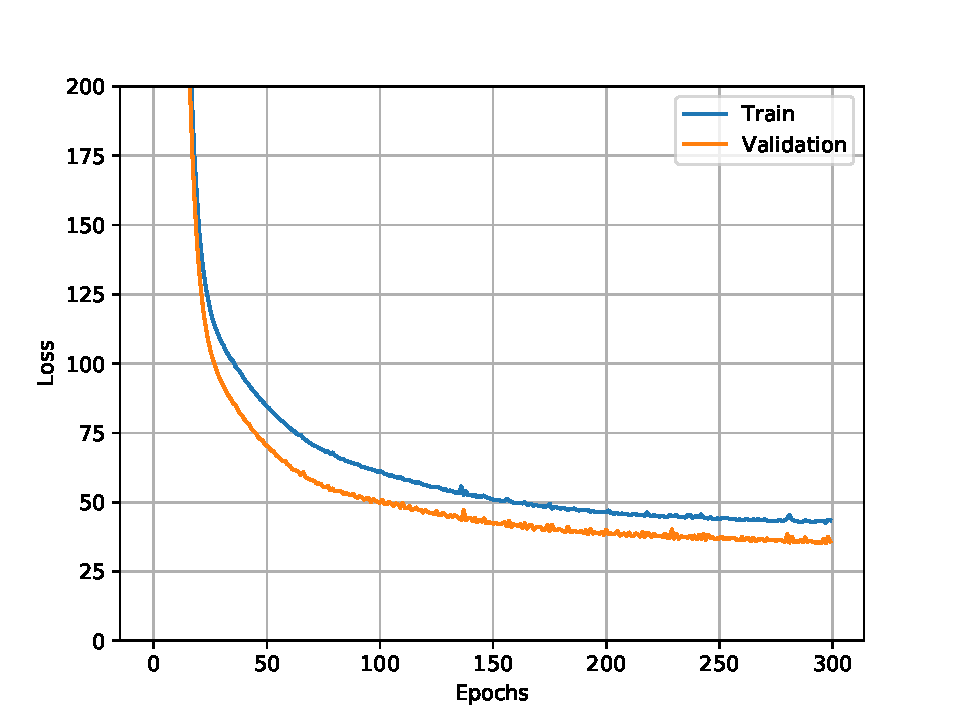
\includegraphics{pics/figure_Boston_NN_1hidden_wd_loss.pdf}
    \caption{Loss on training and validation set during training epochs for the neural network with 1 hidden layers \& weight decay.}
    \label{fig:Boston_NN_1hidden_wd_loss}
\end{figure}


\begin{figure}
    \centering
    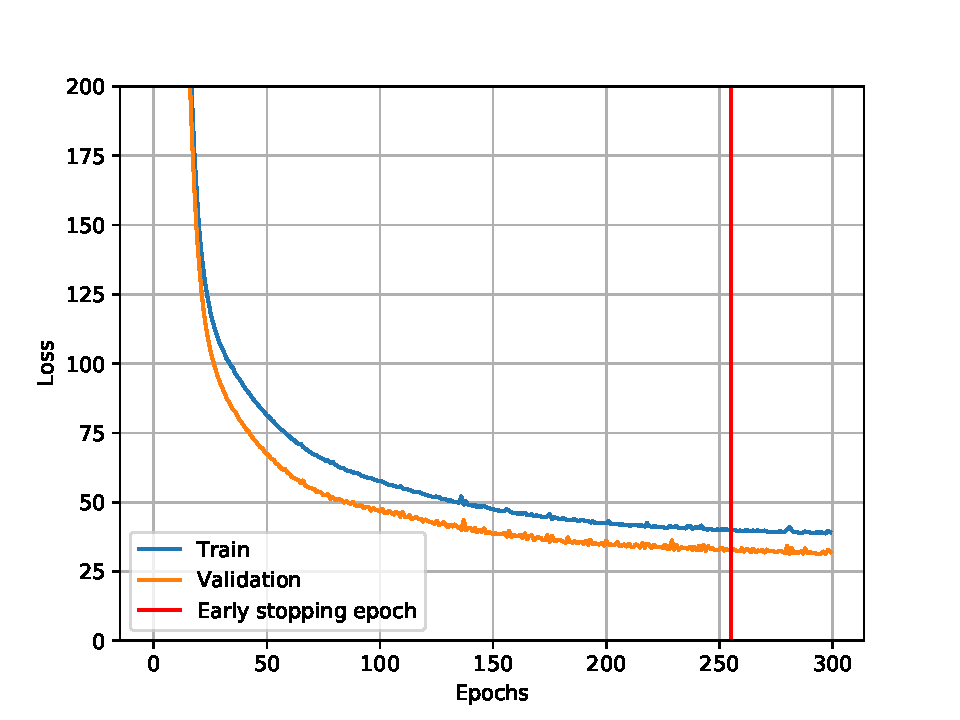
\includegraphics{pics/figure_Boston_NN_1hidden_noreg_loss.pdf}
    \caption{Loss on training and validation set during training epochs for the neural network with 1 hidden layers \& no regularization. These losses are the same as for the network with 1 hidden layer and early stopping up to the stopping time on epoch 255 indicated by the red vertical line. It can be seen that validation loss is somewhat flattening and decreasing in oscillations around epoch 255, which might be what made the early stopping algorithm indicate no further improvements in validation loss, given the chosen patience of 10 epochs and $\delta_{\text{min}} = 0.1$, and stop the training.}
    \label{fig:Boston_NN_1hidden_noreg_loss}
\end{figure}

\begin{table} \label{tab:Boston_NN_performance}
\caption{Performance measurement for Neural Network models on Boston Housing data. Early stopping ran 255 epochs with patience 10 and $\delta_{\text{min}}=0.1$. For weight decay on all networks we select $\alpha = 0.3$ as regularization constant. }
\resizebox{\textwidth}{!}{%
    \begin{tabular}{|l|l|l|l|}
    \hline
    \multicolumn{1}{|c|}{{\cellcolor{ashgrey}{
     \textbf{Model}}}} & \multicolumn{1}{|c|}{{\cellcolor{ashgrey}{
     \textbf{Train MSE}}}}  &\multicolumn{1}{|c|}{{\cellcolor{ashgrey}{
     \textbf{Test MSE}}}}            & \multicolumn{1}{|c|}{{\cellcolor{ashgrey}{
     \textbf{Run time}}}}   \\ \hline
     No hidden layers \& weight decay & 81.798 & 60.074  &   10.64           \\ \hline
    1 hidden layer \& no regularization & 36.539 &  25.650  &   10.14           \\ \hline
    1 hidden layers \& weight decay & 37.103 & 25.542  &   10.81         \\ \hline
    1 hidden layers \& early stopping  & 37.512 & 25.223  &  8.66             \\ \hline
    \end{tabular}
}
\end{table}

\noindent
We examine a network with no hidden layers \& weight decay, as this is equal to linear regression with weight decay. We include this to test if a neural network is beneficial compared to the simple approach of using linear regression. We see from table \ref{tab:Boston_NN_performance} that we get a smaller amount of test and train error when using 1 hidden layer even without regularization, which indicates that using a neural network for this problem is indeed useful.
\\
\\
When we use a neural network with 1 hidden layer and weight decay we get a slightly smaller test loss and slightly larger train loss, than we did when using 1 hidden layer and no regularization, indicating that we might have prevented some overfitting by introducing weight decay. 
\\
\\
We also test regularizing the network of 1 hidden layer by using the method of early stopping, but this gives a slightly larger test loss than the network regularized with weight decay and also slightly larger train loss. It should be noted however that early stopping has decreased the test loss and increased train loss, compared to using no regularization, so the method might still have prevented some overfitting.
Early stopping is, as mentioned in section \ref{sec:early_stopping}, most useful when validation loss begins to increase at some point before ending the training. We see from figure \ref{fig:Boston_NN_1hidden_noreg_loss} that this is not the case, which might explain why early stopping is not as useful as regularizing with weight decay in this case. We examined training periods with more epochs, to see if we might have ended training prematurely, but both validation and training error continued to be around the same level as in epoch 300. 


\subsection{Regression with Bayesian Neural
Networks}





\begin{table}\label{tab:Boston_BNN_performance}
\caption{Performance measurement for Bayesian Neural Network models on Boston housing data}
\resizebox{\textwidth}{!}{%
\begin{tabular}{|l|l|l|l|}
\hline
\multicolumn{1}{|c|}{{\cellcolor{ashgrey}{
\textbf{Model}}}}   &  \multicolumn{1}{|c|}{{\cellcolor{ashgrey}{
 \textbf{Train MSE}}}} & \multicolumn{1}{|c|}{{\cellcolor{ashgrey}{
 \textbf{Test MSE}}}}           & \multicolumn{1}{|c|}{{\cellcolor{ashgrey}{
 \textbf{Runtime (s)}}}}      \\ \hline
No hidden layers &  28.480 &   17.760    &     211.63      \\ \hline
1 hidden layer    &  11.391  & 9.340        &    1496.69                     \\ \hline
Hierarchical with 1 hidden layer     &      14.135          &  10.869  &  1851.46   \\ \hline
\end{tabular}
}
\end{table}

\section{Predicting Default of Credit Card Clients} \label{sec:credit_default}
\subsection{Description and preprocessing of data}
The default of credit card clients data set, contains information, collected by a Taiwan bank in 2005, on $30.000$ credit card clients. The data contains 25 variables, which are represented in table \ref{tab:credit_card_features}. The data set has earlier been used by \cite{Yeh2009TheCO} for predicting the probability of default for customers' in Taiwan and compares the predictive accuracy of probability between six data mining methods. The objective for our analysis is to predict whether a client will default on next month or not. 


\begin{table} \label{tab:credit_card_features}
\caption{Table of features in credit card default data. Data contains 30.000 examples each with 25 features. Data can be downloaded on \href{https://archive.ics.uci.edu/ml/datasets.php}{https://archive.ics.uci.edu/ml/datasets.php}}.
\resizebox{\textwidth}{!}{%
\begin{tabular}{|l|l|}
\hline
\multicolumn{1}{|c|}{{\cellcolor{ashgrey}{
 \textbf{Feature name}}}} & \multicolumn{1}{|c|}{{\cellcolor{ashgrey}{
 \textbf{Feature description}}}}\\ \hline
LIMIT\_BAL                 &           Amount of the given credit (NT dollar): \\ & it includes both the individual consumer credit and \\ &  his/her family (supplementary) credit.           \\ \hline
SEX                        &          Gender (1 = male; 2 = female)            \\ \hline
EDUCATION                  &         Education (1 = graduate school; 2 = university; \\ &  3 = high school; 4 = others).             \\ \hline
MARRIAGE                   &         Marital status (1 = married; 2 = single; 3 = others)             \\ \hline
AGE                        &            Age (year)           \\ \hline
PAY\_0                     &         Repayment status in September, 2005 \\ &  -2=no consumption, -1=pay duly \\ &  0=the use of revolving credit, 1=payment delay for one month \\ &  2=payment delay for two months, 3=payment delay for three months\\ & $\vdots$ \\ &  8=payment delay for eight months, 9=payment delay for nine months and above         \\ \hline
PAY\_2                     &        
Repayment status in August, 2005 (scale same as above)\\ \hline
PAY\_3                     &          Repayment status in July, 2005 (scale same as above)            \\ \hline
PAY\_4                     &            Repayment status in June, 2005 (scale same as above)          \\ \hline
PAY\_5                     &            Repayment status in May, 2005 (scale same as above)          \\ \hline
PAY\_6                     &           Repayment status in April, 2005 (scale same as above)           \\ \hline
BILL\_AMT1                 &           Amount of bill statement in September, 2005 (NT dollar)           \\ \hline
BILL\_AMT2                 &            Amount of bill statement in August, 2005 (NT dollar)          \\ \hline
BILL\_AMT3                 &              Amount of bill statement in July, 2005 (NT dollar)        \\ \hline
BILL\_AMT4                 &            Amount of bill statement in June, 2005 (NT dollar)          \\ \hline
BILL\_AMT5                 &           Amount of bill statement in May, 2005 (NT dollar)           \\ \hline
BILL\_AMT6                 &           Amount of bill statement in April, 2005 (NT dollar)           \\ \hline
PAY\_AMT1                  &               Amount of previous payment in September, 2005 (NT dollar)       \\ \hline
PAY\_AMT2                  &          Amount of previous payment in August, 2005 (NT dollar)            \\ \hline
PAY\_AMT3                  &              Amount of previous payment in July, 2005 (NT dollar)        \\ \hline
PAY\_AMT4                  &              Amount of previous payment in June, 2005 (NT dollar)        \\ \hline
PAY\_AMT5                  &              Amount of previous payment in May, 2005 (NT dollar)        \\ \hline
PAY\_AMT6                  &           Amount of previous payment in April, 2005 (NT dollar)           \\ \hline
default payment next month &             Default payment (1=yes, 0=no)         \\ \hline
\end{tabular}}
\end{table}
\subsection{Classification with Neural Networks}

\begin{table} \label{tab:credit_NN_performance}
\caption{Performance measurement for Neural Network models on Boston Housing data. Early stopping ran 238 epochs.}
\resizebox{\textwidth}{!}{%
    \begin{tabular}{|l|l|l|l|}
    \hline
    \multicolumn{1}{|c|}{{\cellcolor{ashgrey}{
     \textbf{Model}}}} & \multicolumn{1}{|c|}{{\cellcolor{ashgrey}{
     \textbf{Test Accuracy}}}}       & \multicolumn{1}{|c|}{{\cellcolor{ashgrey}{
     \textbf{Run time (s)}}}} & \multicolumn{1}{|c|}{{\cellcolor{ashgrey}{
     \textbf{Accuracy pr. runtime}}}} \\ \hline
    No hidden layers \& weight decay &    &     &          \\ \hline
    1 hidden layer \& no regularization &     &     &          \\ \hline
    1 hidden layers \& weight decay &    &     &          \\ \hline
    1 hidden layers \& early stopping  &     &      &          \\ \hline
    1 hidden layers \& dropout &     &     &          \\ \hline
    \end{tabular}
}
\end{table}

\subsection{Classification with Bayesian Neural Networks}

\begin{table}\label{tab:credit_BNN_performance}
\caption{Performance measurement for Neural Network models on credit card default data}
\resizebox{\textwidth}{!}{%
    \begin{tabular}{|l|l|l|l|l|}
    \hline
    \multicolumn{1}{|c|}{{\cellcolor{ashgrey}{
    \textbf{Model}}}}    & \multicolumn{1}{|c|}{{\cellcolor{ashgrey}{
     \textbf{Train Accuracy (\%)}}}}       & \multicolumn{1}{|c|}{{\cellcolor{ashgrey}{
     \textbf{Test Accuracy (\%)}}}}           & \multicolumn{1}{|c|}{{\cellcolor{ashgrey}{
     \textbf{Run time (s)}}}} & \multicolumn{1}{|c|}{{\cellcolor{ashgrey}{
     \textbf{Accuracy pr. runtime}}}}     \\ \hline
    No hidden layers         &          &               &       &   \\ \hline
    1 hidden layer          &   89.2339     &   84.541             &   2231.83   &    \\ \hline
    Hierarchical with 3 hidden layers     &        &        &      &    \\ \hline
    \end{tabular}
}
\end{table}